\documentclass[fontsize=12bp, paper=a4]{scrarticle}
\usepackage[utf8]{inputenc}
\usepackage[english,main=serbian]{babel}
\usepackage[left=2cm, right=2cm, top=3cm, bottom=3cm]{geometry}
\usepackage[automark]{scrlayer-scrpage}
\usepackage{ragged2e}
\usepackage{amsmath}
\usepackage{mathabx}
\usepackage[colorlinks=true,linkcolor=black,anchorcolor=black,citecolor=black,filecolor=black,menucolor=black,runcolor=black,urlcolor=black]{hyperref}
\usepackage{graphicx}
\usepackage{wrapfig}
\usepackage{amssymb}
\usepackage{listings}
\usepackage{array}
\usepackage{enumitem}
\usepackage{xcolor}
\usepackage{csquotes}
\usepackage{booktabs}
\usepackage{cancel}

%\usepackage[backend=biber, style=numeric]{biblatex}
% kompilirati sa pdflatex-om!
\justifying
%
\definecolor{codegreen}{rgb}{0,0.6,0}
\definecolor{codegray}{rgb}{0.5,0.5,0.5}
\definecolor{codepurple}{rgb}{0.58,0,0.82}
\definecolor{backcolour}{rgb}{0.95,0.95,0.92}

\lstdefinestyle{mystyle}{
    backgroundcolor=\color{backcolour},   
    commentstyle=\color{codegreen},
    keywordstyle=\color{magenta},
    numberstyle=\tiny\color{codegray},
    stringstyle=\color{codepurple},
    basicstyle=\ttfamily\footnotesize,
    breakatwhitespace=false,         
    breaklines=true,                 
    captionpos=b,                    
    keepspaces=true,                 
    numbers=left,                    
    numbersep=5pt,                  
    showspaces=false,                
    showstringspaces=false,
    showtabs=false,                  
    tabsize=2
}

\lstset{style=mystyle}

\renewcommand\lstlistingname{Implementacija}
\renewcommand\lstlistlistingname{Implementacija}

%

\graphicspath{ {./images/} }

%

\title{Seminarski rad} 
\subtitle{iz predmeta Teorijske osnove veštačke inteligencije}

\begin{document}

\begin{titlepage}
    \vspace{\stretch{1}}
    
    \begin{center}
        
        \vspace*{8cm}
        
        \large{Univerzitet u Kragujevcu}
        
        \vspace*{1cm}

        {\bfseries \LARGE Domaći zadatak}
        
        \large{iz predmeta Sistem za podršku odlučivanju}
        
        \vspace*{1cm}
        \large{Tema:}

        \Large{Teorijski izveštaj o regresionim algoritmima sa nadgledanim učenjem}


        \vspace*{2cm}
    \end{center}
    \hfill{\parbox[s]{8cm}{

    mentori: 
    \begin{tabular}{l}
        \\
        \\
        Ognjen Pavić, \\
        prof. dr. Tijana Geroski, \\
        prof. dr. Nenad Filipović 
    \end{tabular}
    
    student: \begin{tabular}{l}
        Željko Simić 3vi/2023
    \end{tabular}
    }}

    \hspace*{\fill} 

    \vspace*{2cm}

    \begin{center}
        Kragujevac 2024.
    \end{center}
\end{titlepage}

\setcounter{page}{1}
\justifying
\linespread{1}
\cfoot[\pagemark]{\pagemark}
\ofoot[]{}
\ohead[]{Željko Simić 3vi/2023}
\chead[]{}
\ihead[]{Univerzitet u Kragujevcu}
%

\section{Uvod}
\subsection{Opis procesa učenja}
Problem obuke obuhvata skupinu $n$ uzoraka podataka i time se pokušava predvideti svojstvo nepoznatih podataka. Ako svaki uzorak ponaosob je više nego 1 unos, npr., multidimenzionalni unos, može se reći da ima više atributa ili features-a.\cite{supervised}
\\
\justifying

Problemi obuke potpadaju u nekoliko kategorija:
\begin{itemize}
    \item \textit{Nenadgledajuće učenje (nije tema ovog rada)} - obuka podacima sastoji se u unosu više vektora $x$ bez ikakvih uparenih ciljnih vrednosti. Cilj je otkriti pripadnost grupi po sličnosti naspram drugih vektora (klasterizacija), ili po raspodeli podataka unutar prostora ulaznih podataka (procena gustine), ili po projekciji podataka višedimenzionog prostora na manje dimenzioni shodnom za vizuelizaciju.
    
    \item \textit{Delimično nadgledano učenje (nije tema ovog rada)\cite{semi}} - situacija gde skup podataka namenjen za obuku ima poneki uzorak koji nije uparen sa ciljanom vrednošću, gde se zarad adekvatnijeg previđanja boljom generalizacijom i distribucijom koriste ciljanom vrednošću nenaznačeni uzorci.
    
    \item \textit{Podsticajuće učenje (nije tema ovog rada)\cite{rl}} - opšti okvir rada gde se vrši obuka \textit{agenata} (tj. algoritma obuke) težeći da se obuče da vrše akcije u zadatom \textit{okruženju} (tj. problema za rešavanje) zarad najboljeg mogućeg slučaja nagrađivanja. 

    \item \textit{\textbf{Nadgledano učenje}} - gde se skup podataka sa prikazanim primerom na slici 1.\cite{dataset} prilaže sa dodatnim atributima po kojim će se predviđanje usmeravati (klasa za svaki od uzoraka, labela). Sastoji se od 2 načina rada (gde samo jednog obrađujemo):
    \begin{itemize}
        \item \textit{Klasifikacija (nije tema rada)} - uzorci mogu da pripadaju dvema (binarna klasifikacija) ili više klasa (višeklasna klasifikacija) i želimo ustanoviti kako bi se predviđanje klasa za nenaznačene podatke vršilo uz pomoć već klasama naznačenih podataka. Način da se sagleda klasifikacija je kao diskretni (suprotno kontinualnom) oblik nadgledane obuke gde od ograničenog broja kategorija za svaki od n uzoraka se namerava dodeliti tačna klasa ili kategorija.
        \item \textit{\textbf{Regresija}} - gde željeni izlaz u priloženom skupu podataka se izražava kao jedna ili više kontinualnih promenljivih, a zadatak predviđanja da nepoznatim ulazima uzorka se naziva regresijom.
    \end{itemize}    
    \begin{figure}[h!]
        \centering
        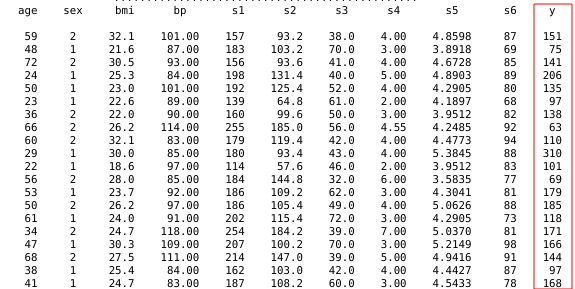
\includegraphics[width=0.75\textwidth]{1.png}
        \caption{\centering Primer skupa podataka - Diabetis, sa atributima \texttt{age,sex,bmi,bp,s1,s2,s3,s4,s5,s6} i targetom \texttt {y} u posebnih 442 uzoraka.}
    \end{figure}
\end{itemize}     

\subsubsection{Trening skup i test skup}
Mašinsko učenje se sačinjava od poduhvata gde se vrši obuka uz svojstva jednog skupa podataka, a vrši testiranje svojstvima uz pomoć nekih drugih skupova podataka. Uobičajena praksa u mašinskom učenju je da se vrši evaluacija algoritma uz podelu skupa podataka na 2 dela. Gde je jedan deo namenjen za obuku (trening skup), a drugi za testiranje (test skup).

\subsubsection{Multiclass vs. multilabel obuka}
Kada se koriste multiklasni klasifikatori, zadaci obuka i predviđanja se izvršavaju tako da zavise od formata podataka ciljanih vrednosti. 1D niz višeklasna labela skupljenih svih uzoraka je moguće navesti da radi \textit{multiklasna predviđanja}. Ciljane vrednosti je moguće mapirati tako da se konvertuju u binarni zapis, tj. niz sastojan od binarnih cifara tako da skup uzoraka ima ciljane vrednosti kao 2d niz i nakon obuke, za obavljana predviđanja smatra se da su \textit{multilabel predviđanja}. Takođe je moguće da ciljana vrednost ima niz više labela (skupljeno po svim uzorcima ciljana vrednost biva 2d niz) za svaki uzorak pri obuci i kasnije naspram toga vršiti predviđanja.

\vbox{}

\subsection{Popularni algoritmi za regresiju}
\justifying
\begin{itemize}
    \item \textbf{Jednostavna linearna regresija (SLR)} - statistički metod koji pomaže pri obuci nad srodnostima među dveju kvantitativnih nezavisnih promenljivih (ulazne \texttt{x} i izlazne \texttt{y}).
    \item \textbf{Višestruka linearna regresija (MLR)} - statistički metod kojim se koristi više raznolikih nekategoričkih nezavisnih promenljivih zarad predviđanja ishoda kontinualne, tj- nekategoričke zavisne promenljive.
    \item \textbf{Polinomijalna linearna regresija (PLR)} - specijalan slučaj MLR-a, obučavanja vrši nad nelinearnim srodnostima među nezavisnim ulaznim i zavisnim izlaznim vrednostima, a oslovljavanje ``linearnom'' je zbog linearnog odnosa koeficijenata $\textbf{b}$ (koji su faktor evaluacije uz ulaznu $\textbf{x}$ promenljivu).
    \item \textbf{Regresija stabla odlučivanja} - cepaju podatke u manje podskupove donesenim odlukama različitim upitima, u isto vreme stablo inkrementalno je razvijeno što ishoduje konačnim čvorovima odluke, ali i čvorovima listova. Radi i sa kategoričkim vrednostima podataka.
    \item \textbf{Regresija slučajne šume} - obuka ansambla koja je moćna tehnika pri unapređivanju modela, gde obuka ansambla podrazumeva kombinovanjem višestrukih evaluacija algoritama zarad formiranja veštog modela optimalnog predviđanja. Zadatak je da regresijom niza više modela stabala odluka kao osnova budu izgrađeni, a pritom obuka bude obavljena agregacijama bootstrapping/bagging-a.
    \item \textbf{Regresija potpornim vektorima (SVR)} - drugačiji oblik mašina potpornih vektora (SVM) i mogu obavljati analize (ne)linearnih regresija na kontinualim vrednostima podataka umesto klasifikacije, koristeći se konceptima hiperravni i granične linije. Naspram drugih algoritama koji minimizuju stopu gubitka, ovi uklapaju gubitak po nekom kriterijumu praga.\cite{algs}
\end{itemize}
U sledećim sekcijama biće obrađivani pomenuti algoritmi.
\newpage
\section{Teorijske osnove i metodologija}
\subsection{Jednostavna linearna regresija (SLR)}
Statistički metod koji pomaže pri obuci nad srodnostima među kvantitativnih promenljivih nezavisnih i zavisnih (ulazne \texttt{x} i izlazne \texttt{y}).

Primer primene SLR-a uključuje procenu plata, stanja tržišta nekretnina, stanja finansijskog portfolija, itd.
Pri proceni kontinualnog izlaza na osnovu jednog ulaza, gde je linearna korelacija vrednosti ulaza i izlaza uzoraka, kao što je prikazano na slici 2. Što je veća vrednost ulaza, veća vrednost izlaza. Uzimaju se u obzir parametri:
\begin{itemize}
    \item $m$ - broj uzoraka trening skupa
    % x = Input Variable/ Feature/ Independent Variable/ Explanatory Variable
    \item $x$ - ulazna promenljiva / feature / nezavisna promenljiva
    % y = Output Variable/ Target Variable/ Dependent Variable
    \item $y$ - izlazna promenljiva / target / zavisna promenljiva
    % (x,y) = One training sample data
    \item $(x,y)$ - opšti oblik uzorka trening podataka
    % (xi, yi) = ith  training example
    \item $(x_i, y_i)$ - i-ti uzorak trening podataka
    \item $y_{predviđenog} - y_i$ - gubitak
    % ypred – yi = Error Difference
\end{itemize}

% Then, the hypothesis of the SLR will be:-
Potom se uzima hipoteza SLR-a:
$$y= a*x + b$$

Target promenljiva $y$ je linearna funkcija promeljive feature-a $x$ i tako je ovo \textbf{univarijantna linearna regresija}.

\begin{figure}[h!]
    \centering
    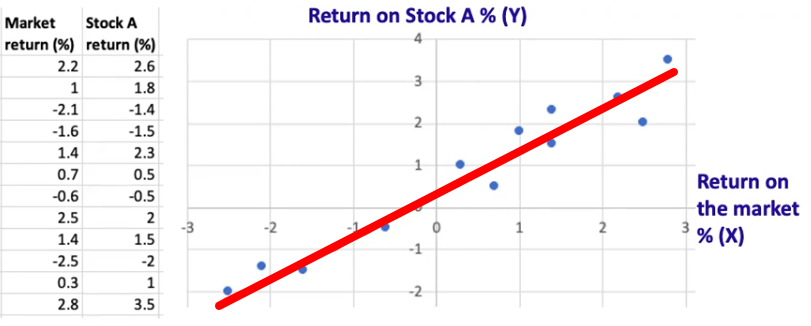
\includegraphics[width=0.75\textwidth]{2.png}
    \caption{\centering Primer skupa podataka - berzanskih akcija, sa atributom \texttt{tržišni povrat na ulog} i targetom \texttt {akcijski povrat na ulog}, pa time određena linija linearne regresije.}
\end{figure}

\subsubsection{Funkcija ocenjivanja i gradijentni spust}
Stremnja linearne regresije je da nađe najbolju moguću vrednost za $a$ (težina parametara u modelu) i $b$ (bias modela) u pomenutoj jednačini.\cite{gfg} \textbf{funkcija ocene} pomoći će da nađemo najbolji ishod tog problema i pritom uklopimo najbolju liniju linearne regresije za uzorke. Ovaj problem se dovodi do potrebe za rešavanjem \textit{problema minimalizacije} gde se minimalizuju gubici između predviđenih i tačnih vrednosti, tj. sa $a$ i $b$ će se \textit{minimalizovati prosečna suma kvadrata grešaka}:
$$
J_{(a,b)} = \frac{1}{2m}\sum_{i=1}^{m} (y_{predviđenog} - y_i)^2
$$

Ovo je poznata \textit{funkcija ocene kvadratnih grešaka}, iliti, \textit{funkcija središnjih kvadratnih grešaka} koja pruža prosečne kvadratne greške nad svim uzorcima skupa podataka. \textit{Gradijentni spust} je metod ažuriranja $a$ i $b$ zarad minimalizacije funkcije ocene $J(a,b)$. Počevši sa $a$ i $b$ postepeno umanjuje se funkcija ocenjivanja korišćenjem diskretnih količina koraka koja je takođe \textit{stope obuke (learning rate) u gradijentnom spustu}. Ovim će biti odlučujuće koliko hipoteza je \textit{brzo konvergira optimalnom minimumu}, prikazano na slici 3. U pythonu biblioteka koja je predodređena za ove  \verb|from sklearn.linear_model import LinearRegression|.

\begin{figure}[h!]
    \centering
    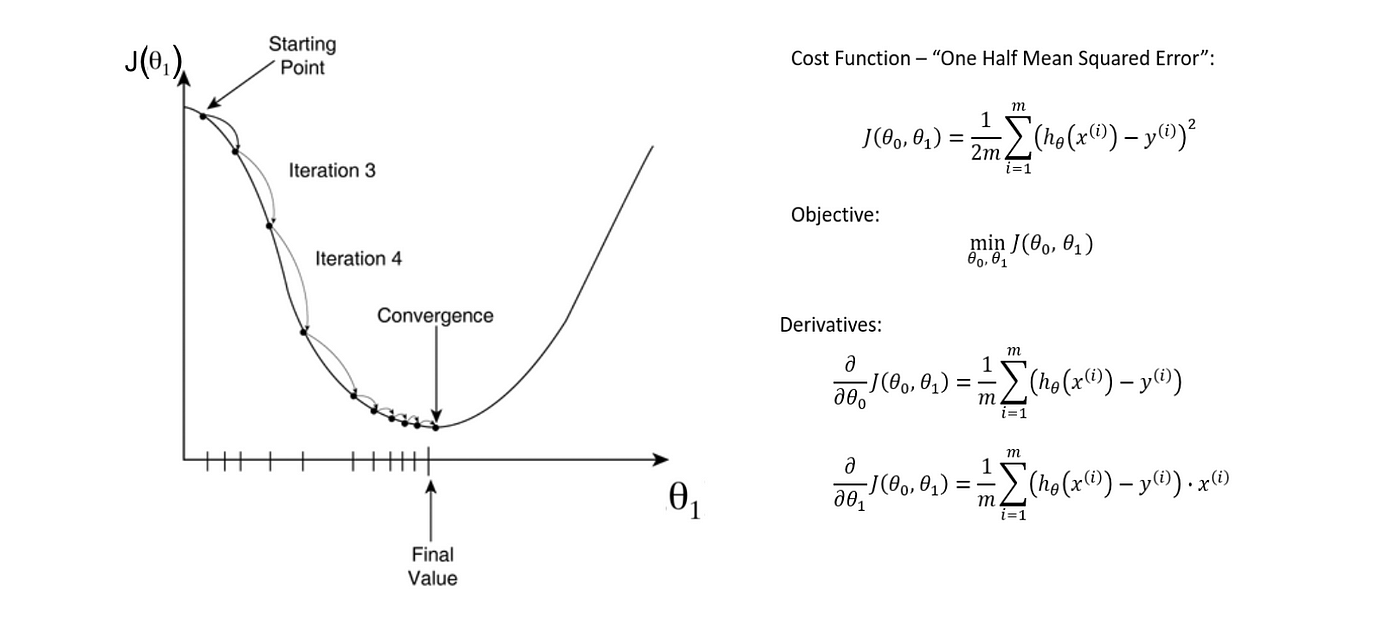
\includegraphics[width=1\textwidth]{3.png}
    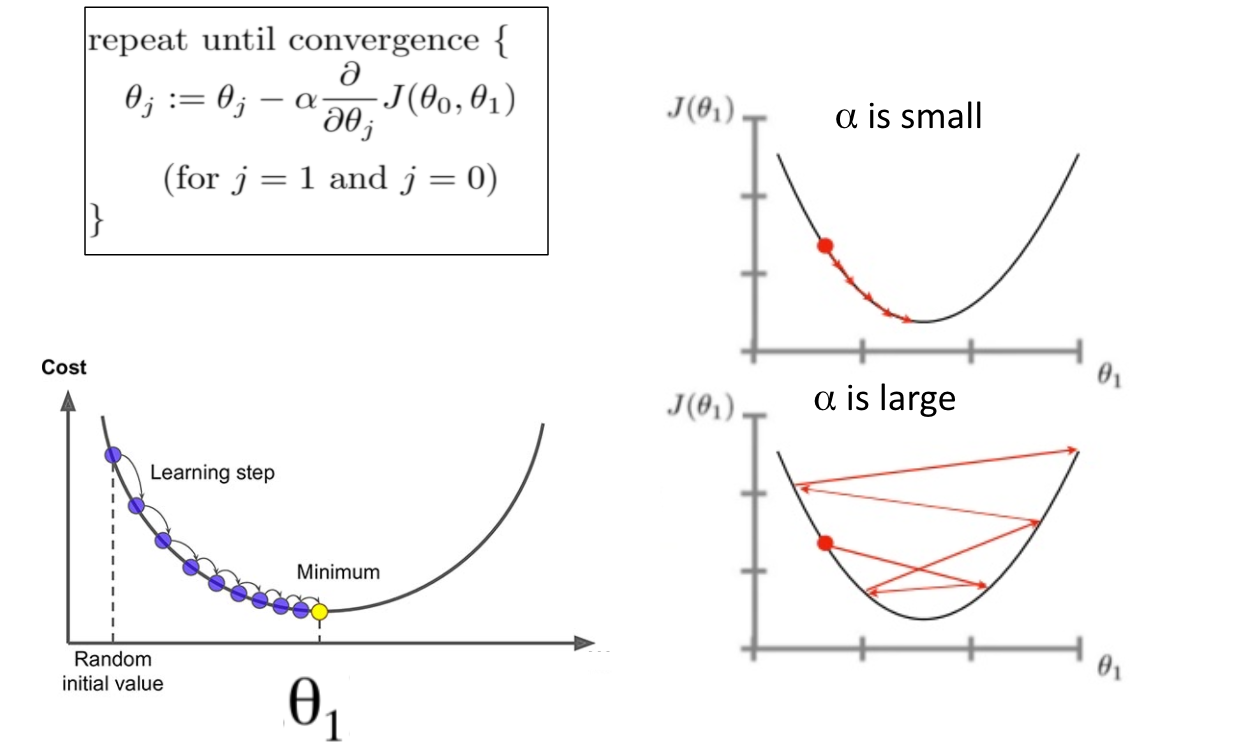
\includegraphics[width=0.75\textwidth]{3b.png}
    \caption{\centering Određivanje funkcije ocenjivanja, kao i algoritamski postupak za slučaj kada je stopa obuke $\alpha$ veća ili mala.}
\end{figure}


% \newpage
\subsection{Višestruka linearna regresija (MLR)}

Ovo je najuobičajeniji oblik analize linearnom regresijom. Statistički metod kojim se koristi više raznolikih nekategoričkih nezavisnih promenljivih (features-a) zarad predviđanja ishoda kontinualne, tj- nekategoričke zavisne promenljive (target-a). Ako su features-i tipa kategoričkih vrednosti tada je neophodno pretvoriti ih u kontinualne promenljive pre korišćenja MLR-a. Stremi se da se nađe linearan odnos medju 2 ili više features-a (oslovljenim kao \textit{prediktor promenljivama}, tj. \textit{regresorima}) i jednom target promenljivom (tzv. \textit{regresandima}).
% MLR Assumptions:
MLR pretpostavke:
\begin{enumerate}
    % 1) Regression Residuals should be normally distributed, homoscedastic and approximately rectangular-shaped.
    \item Odstojanja od regresije bi trebalo biti \textbf{normalno distribuirane} (Gausovom distribucijom, središnja vrednost, specijalan slučaj očekivane vrednosti funkcije distribucije verovatnoća)\cite{mean}\cite{variance}\cite{gaus}, \textbf{homoscendastična} (središnja, tj. očekivana vrednost slučajne promenljive ima \textit{istu} disperziju, tj. varijansu) i \textbf{aproksimirana u pravougaoni oblik}, prikazano na slici 4.
    
    \begin{figure}[h!]
        \centering
        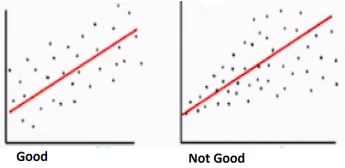
\includegraphics[width=0.5\textwidth]{4.png}
        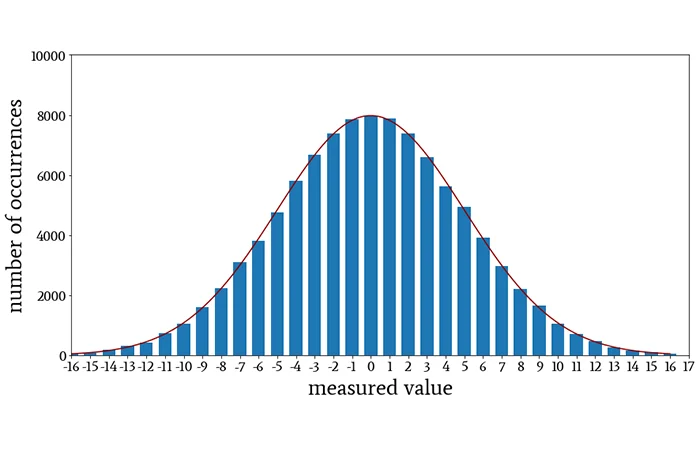
\includegraphics[width=0.5\textwidth]{4a.png}
        \caption{\centering Homoscendastičnost ostvarena i neostvarena. Gausova distribucija, aproksimirana u pravougaoni oblik.}
    \end{figure}
    % 2) A linear relationship is assumed between the independent variables and the dependent variable.
    \item Linearan odnos se nagađa među promenljivama features-a i target promenljivoj.
    % 3) Lack of multicollinearity which means that the independent variables are not highly correlated to each other.
    \item Izostajanje višestruke kolinearnosti koja označava da features-i nisu blisko srodni međusobno.\cite{colinear}
    % 4) Adding too much independent variable will increase the amount of explained variance in the dependent variable (also known as R-squared, R2 or co-efficient of determination) and it will result in an over-fit model.
    \item Dodavanje previše features-a će uvećati količinu \textit{objašnjavajuće disperzije} 
    $$explained\_{}variance(y, \hat{y}) = 1 - \frac{Var\{ y - \hat{y}\}}{Var\{y\}}$$
     po promenljivi targeta (takođe postoji R2 ocena, koeficijent determinizma, 
     $$R^2(y, \hat{y}) = 1 - \frac{\sum_{i=1}^{n} (y_i - \hat{y}_i)^2}{\sum_{i=1}^{n} (y_i - \bar{y})^2},$$ gde $\hat{y}_i$ je predviđena target vrednost, a $\bar{y}$ je očekivana vrednost, koja ukazuje na doslednost obuke i mera je koliko neuvaženih uzoraka će biti predviđeno modelom i predstavljena je na slici 5.)\cite{explainedVar}\cite{r2}\cite{hat} i rezultovaće da model ode u stanje overfitting-a.

    \begin{figure}[h!]
        \centering
        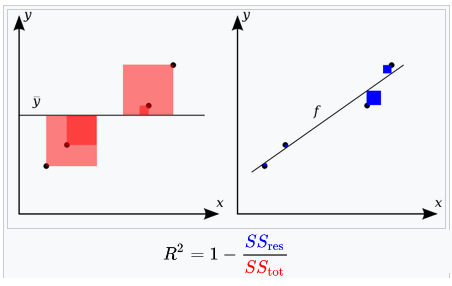
\includegraphics[width=0.5\textwidth]{5.png}
        \caption{\centering R2 skor vizuelizacija uticaja postupka.}
    \end{figure}
\end{enumerate}


MLR koristi se:
\begin{enumerate}
    \item pri identifikaciji doprinosa features promenljivih na target promenljivu;
    \item pri prognoziranju promene kod target promenljive sa promenama promljenivih features-a;
    \item pri predviđanju trendova i budućih vrednosti na tržištu.
\end{enumerate}


% MLR Intuition:

Formula MLR-a je $y =  b_0 + b_1x_1 + b_2x_2 + b_3x_3 + \dots + b_nx_n$, gde postoji $n+1$ features promenljivih, $y$ target promenljiva, $x_1, x_2, x_3, \dots ,x_n$ features-i, $b_0$ je odsečak na y-osi, $b_1, b_2, b_3, \dots, b_n$ koeficijenti nagiba za svaku promenljivu features-a, kao na slici 6.
\begin{figure}[h!]
    \centering
    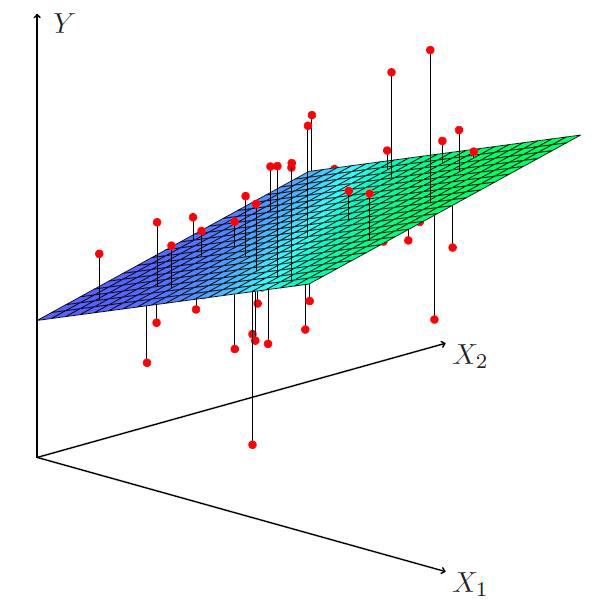
\includegraphics[width=0.25\textwidth]{6.png}
    \caption{\centering Višestruka linearna regresija.}
\end{figure}
MLR je primenjen da odredi linearni matematički odnos među nekolicini slučajnih promenljivih zarad formiranja linije prave koja najbolje aproksimira sve tačke uzoraka skupa podataka u multidimenzionalnom prostoru. 

Za implementaciju u python-u koriste se moduli:
\begin{itemize}
    \item \verb|from sklearn.preprocessing import LabelEncoder, OneHotEncoder| za enkodiranje labele promenljive targeta i promenljivih features-a,
    \item a regresija je obavljena uz modul \verb|from sklearn.linear_model import LinearRegression|.
\end{itemize}

\newpage
\subsection{Polinomijalna linearna regresija (PLR)}
Specijalan slučaj MLR-a, obučavanja vrši nad nelinearnim srodnostima među nezavisnim ulaznim i zavisnim izlaznim vrednostima, a oslovljavanje ``linearnom'' je zbog linearnog odnosa koeficijenata $\textbf{b}$ (koji su faktor evaluacije uz $\textbf{x}$). Target promenljiva $y$ je definisana kao n-ti stepen polinom po feature promenljivoj $x$. Teži se da se obuči tačkama uzoraka model sa najboljim mogućim vrednostima koeficijenata.

Hipoteza PLR-a je data formulom
$$ y = b_0 + b_1x_1 + b_2x_1^2 + b_3x_1^3 + \dots + b_nx_1^n,$$
gde je $y$ target promenljiva, $x_1, x_1^2, x_1^3, \dots, x_1^n$ feature promenljiva za član svakog stepena, $b_0, b_1, b_2, \dots, b_n$ koeficijenti promenljive feature-a za član svakog stepena.

\begin{figure}[h!]
    \centering
    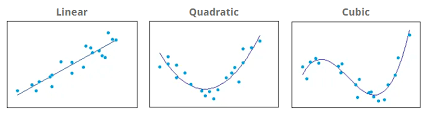
\includegraphics[width=1\textwidth]{7.png}
    \caption{\centering PLR za linearni, kvadtni i kubni slučaj.}
\end{figure}

PLR je korišćen kada linija prave iz SLR ili MLR nije skladna pri obuci tačaka uzoraka skupa podataka i potrebna je parabolička kriva 2. reda pri takvoj obuci. Polinomijalni član stepena 2. (kvadratnog) ili 3. (kubnog) pretvaraju linearni regresioni model u krivu 2. reda i slika 7. to prikazuje. Pri sagledanju tačaka uzoraka skupa podataka promenljivom features-a i target-a koje su razbacane ili u odnosu krivolinijskom najbolje je koristiti PLR s obzirom da na takvom tipu podataka time će se rezultovati više negativnim i pozitivnim odstojanjima.

Moguće je naići na problem overfittinga pri određivanju regresije uz povećavanje stepena polinomijalne regresije zarad dostizanja sve bolji ishod modela.\cite{gfgRegr} Tako po nastalom overfittingu nove tačke uzoraka skupa podataka ne bivaju obrađene. 

Ovim povodom pri regresiji biće pokušaja da se penalizuju težine (koeficijenti) modela zarad regularizacije efekta problema overfitting-a. Tehnike regularizacije koje su dostupne kao metodologije su \textit{Lasso regresija} i \textit{Ridge regresija}.

Generalizacija pristupa odlučivanja da li će se dati prednost bias-u ili disperziji da se zaobiđu problem underfitting-a i overfitting-a kojeg obrađujemo uz selekciju adekvatne vrednosti za stepen polinoma po kom se obuka nad podacima vrši. Stepen polinoma koji je povećan nakon početka rasta određenog nivoa razmaka trening i validacionih metrika.

U python-u modul koji se koristi za ovaj model je:
\begin{itemize}
    \item \verb|from sklearn.preprocessing import PolynomialFeatures|,
    \item \verb|from sklearn.linear_model import LinearRegression|.
\end{itemize}

\newpage
\subsection{Regresija stabla odlučivanja}
Korišćena da previđaju target vrednost po uzetim za obuku pravilima odlučivanja naspram features-a. Stablo odlučivanja pri vršenju regresije nad modelom gradi strukturu stabla, kao što je prikazano na slici 8. Cepaju podatke u manje podskupove donesenim odlukama različitim upitima, u isto vreme stablo inkrementalno je razvijeno što ishoduje konačnim \textit{čvorovi odluke}, ali i \textit{čvorovi listova}. Radi i sa kategoričkim vrednostima podataka. Ovo je tehnika koja je nelinearni, nekontinualni regresioni model.

\begin{figure}[h!]
    \centering
    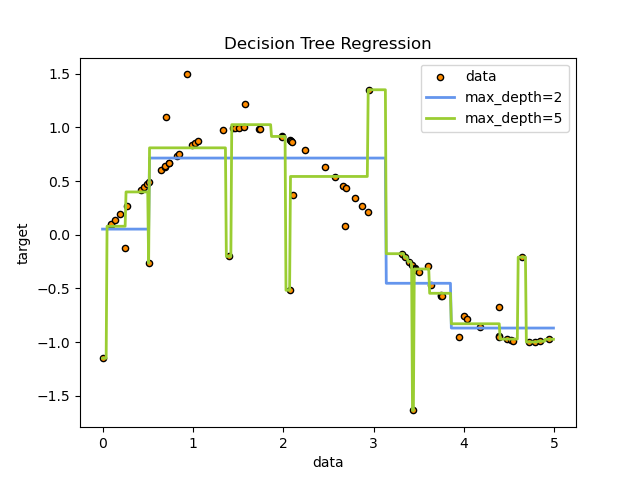
\includegraphics[width=0.5\textwidth]{8.png}
    \caption{\centering Regresija stablom odlučivanja.}
\end{figure}

Za čvor odluke koji može imati 2 grane gde svaka ističe testirane vrednosti atributa. Čvor lista ističe odluku na numeričku vrednost target promenljive. Najuzvišeniji čvor odluke u stablu ističe najboljeg predviđivača koji je tzv. \textit{čvor korena} (prvi roditelj).

Stablo odlučivanja je konstruisano procesom \textit{rekurzivnog particionisanja} počev od čvora korena. Svaki čvor može biti deljen naspram levog i desnog čvora potomka koji mogu se dalje i oni deliti. Ovi čvorovi će postati čvorovi roditelji za njihove ishodujuće potomke čvorove. Cilj ove procedure je da ispuni kriterijum da minimizuje ustanovljene lokacije za buduće podele koji je \textit{središnja kvadratna greška (MSE, L2 greška), Poasonovu devijaciju}, \textit{središnja apsolutna greška (MAE ili L1 greška)}.\cite{dTree} MSE i Poasonova devijacija obe predviđaju vrednost čvorova listova za ustanovljenu središnju vrednost $\bar{y}_m = \frac{1}{n_m}\sum_{y \in Q_m} y$ za čvor $m$, gde je za MAE predviđena vrednost čvora lista na medianu $median(y)_m$.

\begin{itemize}
    \item MSE se računa kao: $H(Q_m) = \frac{1}{n_m} \sum_{y \in Q_m} (y - \bar{y}_m)^2$,
    \item Prepolovljena Poasonova devijacija kao: $H(Q_m) = \frac{1}{n_m} \sum_{y \in Q_m} (y \log\frac{y}{\bar{y}_m} - y + \bar{y}_m)$.
    Poasonova devijacija je pogodna ako je target frekvencija ili količina, ali, u svakom slučaju, $y >= 0$ je uslov da bi se ona koristila kao kriterijum. Obučava sporije od MSE.
    \item $H(Q_m) = \frac{1}{n_m} \sum_{y \in Q_m} |y - median(y)_m|$, gde je $median(y)_m = \underset{y \in Q_m}{\mathrm{median}}(y)$. Obučava sporije od MSE.
\end{itemize}

Implementacija u python-u je vršena uz korišćenje modula:

\verb|from sklearn.tree import DecisionTreeRegressor|.

\newpage
\subsection{Regresija slučajne šume}
Obuka ansambla koja je moćna tehnika pri unapređivanju modela, gde obuka ansambla podrazumeva kombinovanjem višestrukih evaluacija algoritama zarad formiranja veštog modela optimalnog predviđanja.

% Regression and Classification tasks by combining decisions from a sequence of multiple base 
Kao metod ansambla obavlja zadatke regresija kombinujući odluke iz niza više modela stabla odluka u osnovi. I njihovo matematičko tumačenje je da:
$$g(x) = f_0(x) + f_1(x) + f_2(x) + \dots + f_n(x),$$
gde konačni ansamblov model regresije slučajnih šuma $g(x)$ je suma običnih modela stabala odlučivanja u osnovi $f_n(x)$. Posebno modeli stabla odlučivanja su konstruisani nezavisnim različitim poduzorcima trening skupa i ovaj proces treniranja svakog stabla odluke sa različitim uzorcima skupa podataka, gde je uzorkovanje urađeno sa zamenom, je poznato kao \textit{Bagging/Bootstrap agregacija}.

Koristan je pri regresiji skupa podataka sa numeričkim i kategoričkim features-ima naspram drugih regresija. Za razliku od ostalih linearnih regresionih modela, regresije slučajnih šuma mogu da obuhvate nelinearnu interakciju među promenljivama features-a i promeljive target-a.

Ne radi efikasno sa raspršenim vrednosti promenljivih features-a, obično kategoričkog tipa višedimenziono. Neophodna je ili predobrada nad features-ima da se generišu numeričke vrednosti, ili primena linearnog modela.

% Steps to build a Random Forest Regression Model
Za izgradnju modela za regresiju slučajnih šuma (kao na slici 9.) prate se koraci:
\begin{enumerate}
    \item Odabrati nasumičnih $n$ uzoraka trening skupa;
    \item Gradi se u osnovi model stabla odlučivanja uvaženih za $n$ uzoraka skupa podataka;
    \item Odabrati nekih $N$ stabal odlučivanja koja će biti konstruisana;
    \item Ponoviti korak 1. i korak 2. $N$ puta;
    \item Za novu tačku uzorka skupa podataka, napravi se $N$ ustanovljenih predviđanja vrednosti od stabala odlučivanja i odrediti \textbf{prosečnu vrednost} svih vrednosti predviđenih izlaza nove tačke uzorka.
\end{enumerate}


\begin{figure}[h!]
    \centering
    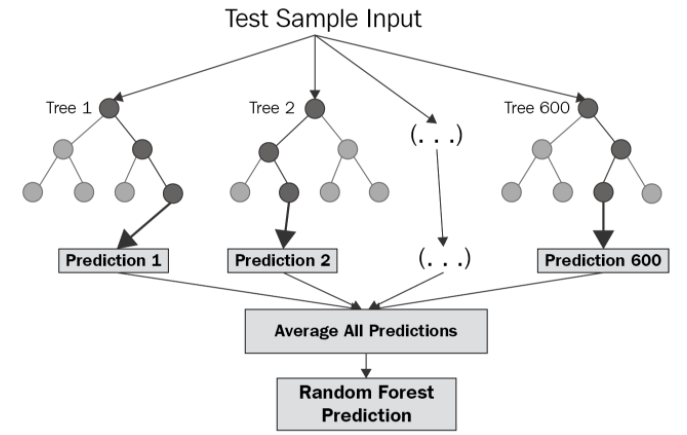
\includegraphics[width=0.42\textwidth]{9.png}
    \caption{\centering Regresija slučajnom šumom.}
\end{figure}

Za implementaciju korišćeni su moduli:
\begin{itemize}
    \item \verb|from sklearn.ensemble import RandomForestRegressor|
    \item \verb|from sklearn.preprocessing import LabelEncoder|
\end{itemize}

\newpage
\subsection{Regresija potpornim vektorima (SVR)}
Drugačiji oblik mašina potpornih vektora (SVM) i mogu obavljati analize (ne)linearnih regresija na kontinualim vrednostima podataka umesto klasifikacije, koristeći se konceptima \textbf{hiperravni} i \textbf{granične linije}, uzimajući u obzir dijagrama na slici 10. (hiperravan je plava, a granične linije su crvene). Naspram drugih algoritama koji minimizuju stopu gubitka, ovi uklapaju gubitak po nekom kriterijumu praga.


\begin{figure}[h!]
    \centering
    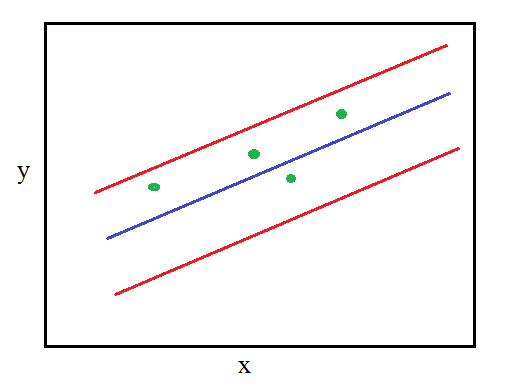
\includegraphics[width=0.5\textwidth]{10.png}
    \caption{\centering Regresija potpornim vektorom.}
\end{figure}

SVR podržava (ne)linearne regresije i tako pokušava obučiti sa što više uzoraka skupa podataka moguće koja je ostvarena usput plavim i crvenim linijama ograničavajući margine prekršavanja. SVR vrši regresiju u višedimenzionom prostoru i svaki posebno uzorak predstavlja svoju sopstvenu dimenziju. Širina među crvenim linijama i plavom linijom je kontrolisana je uz \textbf{hiperparametar $\epsilon$}. Stremnja SVR modela je da uzme u obzir uzorke unutar oblasti između crvenih linija i najbolja obuka je ostvarena na plavoj hiperravni koja će imati maksimalni broj uzoraka.

Kada se vrši evaluacija kernela među uzorcima trening skupa i uzorcima test skupa, rezultujuća vrednost daje koordinatu uzorka test skupa u toj dimenziji. Vektor k proizveden kada tačka uzorka test skupa je evaluirana za sve tačke uzoraka trening skupa i tumači se kao tačka test skupa u višedimenzionim prostorima. Ovaj vektor može biti korišćen da obavi linearnu regresiju. Vektori najbliži tački test skupa su oslovljeni kao {potporni vektori}.

Da bi se obavila obuka SVR modela, moramo imati trening skup, koji pokriva oblast interesa i podstaknut je rešenjima u ovoj oblasti. Posao SVR-a je da aproksimira funkciju koju koristimo da generišemo obuku trening skupom. Nakon pribavljanja trening skupa, moramo odabrati \textbf{kernel}, njegove parametre i neki potrebna \textbf{regularizacija $C$}-om. Onda, moramo ostvariti \textbf{matricu korelacija} i obučiti model da dobavi \textbf{kontrakcione koeficijente}. Korišćenjem ovih koeficijenata, moguće je generisati poseban procenjivač.

Za implementaciju u python-u koristi se modul \verb|from sklearn.svm import SVR|.

\newpage

\section{Diskusija o algoritmima}
\subsection{Prednosti i mane}
\subsubsection{Jednostavna linearna regresija}
% Advantages of Linear Regression
\textbf{Prednosti jednostavne linearne regresije:\cite{slr}} 
\begin{itemize}
    %     Linear regression is a relatively simple algorithm, making it easy to understand and 
    \item Linearna regresija je relativno jednostavan algoritam što ga čini lakim za razumevanje i implementiranje;
    %     implement. The coefficients of the linear regression model can be interpreted as the 
    %     change in the dependent variable for a one-unit change in the independent variable, 
    \item Koeficijentima modela linearne regresije može biti protumačena promena u target promenljivoj za jednu jediničnu vrednosnu promenu u feature promenljivoj što daje uvid u korelaciju među promenljivama;
    %     providing insights into the relationships between variables.
    %     Linear regression is computationally efficient and can handle large datasets 
    %     effectively. It can be trained quickly on large datasets, making it suitable for 
    \item Linearna regresija je računski efikasna i može rukovati ogromnim skupovima podataka efikasno;
    %     real-time applications.
    \item Može biti obučena brzo na velikim skupovima podataka, što je čini adekvatnom za primene u realnom vremenu;
%     Linear regression is relatively robust to outliers compared to other machine learning 
    \item Linearna regresija je relativno robustna što se tiče outliers-a u poređenju sa algoritmima mašinskog učenja.  Outliers-i mogu imati manji uticaj na sveukupne performase modela;
%     algorithms. Outliers may have a smaller impact on the overall model performance.
%     Linear regression often serves as a good baseline model for comparison with more complex 
    \item Linearna regresija često služi dobrim baseline model (bez ikakvih inicijalnih konfiguracija parametara) za poređenje više složenijih algoritama mašinskog učenja;
%     machine learning algorithms.
%     Linear regression is a well-established algorithm with a rich history and is widely 
    \item Linearna regresija je dobro ustanovljen algoritam sa bogatom istorijom i široko je dostupna u raznovrsnim softverskim bibliotekama mašinskog učenja.
%     available in various machine learning libraries and software packages.
\end{itemize}
\textbf{Mane jednostavne linearne regresije:}
% Disadvantages of Linear Regression
\begin{itemize}
    %     Linear regression assumes a linear relationship between the dependent and independent 
    %     variables. If the relationship is not linear, the model may not perform well.
    \item Linearna agresija nagađa linearnu srodnost između target i feature promenljivih. Ako odnos je nelinearan, model se neće dobro pokazati pri obavljanju posla;
    %     Linear regression assumes that the features are already in a suitable form for the 
    \item Linearna regresija nagađa da feature je i inače u pogodnom obliku za model;
    %     model. Feature engineering may be required to transform features into a format that can 
    \item Neophodno je neko prilagođavanje feature-a tako da se obavlja preoblikovanje feature-a u format koji može biti efektivno korišćen od modela;
    %     be effectively used by the model.
    %     Linear regression is susceptible to both overfitting and underfitting. Overfitting 
    %     occurs when the model learns the training data too well and fails to generalize to 
    %     unseen data. Underfitting occurs when the model is too simple to capture the underlying 
    %     relationships in the data.
    \item Linearna regresija je podložna da ode u stanje overffiting-a i underfitting-a. Overfitting nastaje kada model uči iz trening skupa toliko detaljno da ne uspeva da izopšti nesagledane podatke. Underfitting nastaje kada model je jednostavan da obuhvati uspostavljene odnose u skupu podataka;
    %     Linear regression provides limited explanatory power for complex relationships between 
    \item Linearna regresija ustupa ograničenu moć pojašnjavanja složenih odnosa među promenljivama. Što su tehnike mašinskog učenja naprednije to su neophodni produbljeni uviđaji.
    %     variables. More advanced machine learning techniques may be necessary for deeper 
    %     insights.
\end{itemize}

% https://sciencing.com/advantages-disadvantages-multiple-regression-model-12070171.html
\subsubsection{Višestruka linearna regresija}
% Advantages of Linear Regression
\textbf{Prednosti višestruka linearna regresija:\cite{mlr}} 
% Advantages of Multiple Regression
\begin{itemize}
    % There are two main advantages to analyzing data using a multiple regression model. The first is the ability 
    % to determine the relative influence of one or more predictor variables to the criterion value. The real estate 
    \item Mogućnost zaključivanja uticaja 1 ili više feature promenljivih na target vrednost. 
    
% agent could find that the size of the homes and the number of bedrooms have a strong correlation to the price 
% of a home, while the proximity to schools has no correlation at all, or even a negative correlation if it is 
% primarily a retirement community.
% % The second advantage is the ability to identify outliers, or anomalies. For example, while reviewing the data 
    \item Identifikuju outliers-e ili anomalije.
% related to management salaries, the human resources manager could find that the number of hours worked, the 
% department size and its budget all had a strong correlation to salaries, while seniority did not. 
% Alternatively, it could be that all of the listed predictor values were correlated to each of the salaries 
% being examined, except for one manager who was being overpaid compared to the others.
\end{itemize}
% % Disadvantages of Multiple Regression
\textbf{Mane višestruke linearne regresije:}
   
    
\begin{itemize}
    \item Linearna regresija je osetljiva na multikolinearnost, što se ističe kada je visoka korelacija među feature promenljivama;

    \item Multikolinearnost može uvećati disperziju koeficijenata i dovesti do nestabilnih predviđanja modela;
    \item Mogućnost loših performansi pri nedostajućim vrednostima.

\end{itemize}

% https://www.geeksforgeeks.org/python-implementation-of-polynomial-regression/#advantages-disadvantages-of-using-polynomial-regression
\subsubsection{Polinomijalna linearna regresija}
\textbf{Prednosti polinomijalna linearna regresija:\cite{plr}} 
\begin{itemize}
% Advantages of using Polynomial Regression
%     A broad range of functions can be fit under it.
    \item Širok opseg funkcija može biti korišćen obuku;
    %     Polynomial basically fits a wide range of curvatures.
    \item Obično obuku vrši nad širokim opsegom krivih 2. reda;
    %     Polynomial provides the best approximation of the relationship between dependent and independent variables.
    \item Prilaže najbolje aproksimacije srodnosti među target i nezavisnim promenljivama.
\end{itemize}
\textbf{Mane višestruke linearne regresije:}
\begin{itemize}

% Disadvantages of using Polynomial Regression 

%     These are too sensitive to outliers.
    \item Preosetljive na outliers-e;
    %     The presence of one or two outliers in the data can seriously affect the results of nonlinear analysis.
    \item Prisutnost 1-2 outliers-a u skupu podataka mogu ozbiljno uticati na rezultate nelinearne analize;
    %     In addition, there are unfortunately fewer model validation tools for the detection of outliers in nonlinear regression than there are for linear regression.
    \item Pristuno je mali broj alata za validaciju za detekciju outliers-a u nelinearnoj regresiji nego što ih ima za linearnu regresiju.
\end{itemize}


% https://www.geeksforgeeks.org/pros-and-cons-of-decision-tree-regression-in-machine-learning/
\subsubsection{Regresija stabla odlučivanja}
\textbf{Prednosti regresija stabla odlučivanja:\cite{dtreeplusminus}} 
\begin{itemize}
% Pros of Decision Tree Regression
%     Interpretability: One of the significant advantages of decision trees is their interpretability. The decision rules learned by the algorithm are easy to understand and visualize, making it simple to explain to non-technical stakeholders. This transparency is valuable in domains where interpretability is crucial, such as finance or healthcare.
    \item Jasnost pravila odlučivanja bivaju učena od strane algoritma, omogućuju razumljivost i vizuelizaciju, pored toga ustupaju moć lakog pojašnjavanja nestručnim licima;
%     Non-linear relationships: Decision trees can capture non-linear relationships between features and the target variable. Unlike linear models, decision trees can represent complex decision boundaries, making them suitable for datasets with intricate patterns.
    \item Nelinearni odnosi između features-a i target promenljive koji su obuhvaćeni stablom odlučivanja; Za razliku od linearnih modela, stabla odlučivanja mogu reprezentovati složene granice odluke, njihovim uspostavljanjem prilagođeni su za skupove podataka sa složenijim obrascima.
%     No feature scaling required: Decision trees are not sensitive to the scale of features, meaning there’s no need for feature scaling (e.g., normalization or standardization) as required by some other algorithms like Support Vector Machines or K-Nearest Neighbors.
    \item Skaliranje (normalizacija ili standardizacija) features-a nije potrebno pošto stabla odlučivanja nisu osetljiva na raspone features-a.
%     Handles both numerical and categorical data: Decision trees can handle both numerical and categorical features without the need for one-hot encoding or other preprocessing techniques. This makes them convenient for datasets with mixed data types.
    \item Rukuje i sa numeričkim i kategoričkim podacima (bez ikakvih one-hot enkodiranja ili drugih tehnika predobrada). Ovo ih čini pogodnim za skupove podataka sa izmešanim tipovima podataka.
%     Robust to outliers: Decision trees are robust to outliers in the data. Since they partition the feature space into regions based on the values of features, outliers tend to have minimal impact on the overall model performance.
    \item Robustni na outliers-e u podacima. Počeviši od njihovog particionisanja feature prostora u regione zasnovane na vrednostima features-a, outliers-i streme da imaju minimalni uticaj na sveukupnu performansu modela.
\end{itemize}
\textbf{Mane višestruke linearne regresije:}
\begin{itemize}
% Cons of Decision Tree Regression
%     Overfitting: Decision trees are prone to overfitting, especially when they grow too deep or when the dataset is noisy. Deep decision trees can memorize the training data, leading to poor generalization on unseen data. Techniques like pruning or limiting the tree depth can mitigate this issue.
\item Overfitting-u podložno, pogotovo pri produbljenosti stabla ili je skup podataka raspršen.
%     High variance: Decision trees have high variance, meaning small changes in the training data can result in significantly different trees. Ensemble methods like Random Forest or Gradient Boosting are often used to reduce variance and improve performance.
\item Visok nivo disperzije je prisutan, jer male izmene u trening skupu mogu rezultovati značajno različitim stablima;
%     Instability: Decision trees are sensitive to small variations in the data, which can lead to different splits and, consequently, different trees. This instability makes them less reliable compared to some other algorithms.
\item Nestabilnost pošto je osetljivost velika za male promene u podacima, što vodi u različite podele i posledično drugačija stabla, a to ih čini manje pouzdanim naspram drugih algoritama;
%     Bias towards features with many levels: Features with a large number of levels (i.e., high cardinality) tend to be favored over features with fewer levels in decision tree splits. This bias can affect the performance of the model, especially if the high-cardinality features are not truly informative.
\item Bias naspram features-a, tj. za visok nivo (tj. visok broj uzoraka) može dovesti do pristrasnosti naspram features-a sa manjim nivoima u podelama stabla odlučivanja;
%     Difficulty in capturing linear relationships: Despite being able to capture non-linear relationships, decision trees struggle with capturing linear relationships between features and the target variable. Other algorithms like linear regression may perform better in such cases.
\item Težina u prikupljanju linearnih srodnosti, iako je shodan uhvatiti nelinearne srodnosti, stablo odlučivanja ima ovu problematiku za srodnosti među features-ima i target promenljom. 
\end{itemize}

% https://www.geeksforgeeks.org/random-forest-regression-in-python/
\subsubsection{Regresija slučajnih šuma}
\textbf{Prednosti regresija slučajnih šuma:\cite{rfr}} 
\begin{itemize}
% Advantages of Random Forest Regression
%     It is easy to use and less sensitive to the training data compared to the decision tree.
\item Lako je koristiti i manje je osetljiva naspram trening skupa;
%     It is more accurate than the decision tree algorithm.
\item Tačniji za razliku od stabala odlučivanja;
%     It is effective in handling large datasets that have many attributes.
\item Efektivniji u baratanju ogromnim skupovima podataka koji imaju više atributa;
%     It can handle missing data, outliers, and noisy features.
\item Barataju nedostajućim podacima, outliers-ima, šumovima u features-ima.
\end{itemize}

% Disadvantages of Random Forest Regression
\textbf{Mane višestruke linearne regresije:}
\begin{itemize}
    %     The model can also be difficult to interpret.
    \item Teško rastumačiv;
    %     This algorithm may require some domain expertise to choose the appropriate parameters like the number of decision trees, the maximum depth of each tree, and the number of features to consider at each split.
    \item Zahteva neka poznavanja u stučnoj oblasti zarad odabira odgovarajućih parametara kao što su: broj stabala odlučivanja, maksimalna dubina drveta, broj features-a za uzimanje u obzir svakom podelom;
    %     It is computationally expensive, especially for large datasets.
    \item Računski je skup, pogotovo za ogromne skupove podataka;
    %     It may suffer from overfitting if the model is too complex or the number of decision trees is too high.
    \item Ispašta po pitanju overfitting-a ako model je previše složen ili broj slučajnih stabala je previsok.
\end{itemize}

% https://towardsdatascience.com/unlocking-the-true-power-of-support-vector-regression-847fd123a4a0
\subsubsection{Regresija potpornim vektorima}
\textbf{Prednosti regresija potpornim vektorima:\cite{svr}} 
\begin{itemize}
    % Advantages of Support Vector Regression
    
    % Although Support Vector Regression is used rarely it carries certain advantages that are as mentioned below:
    
    %     It is robust to outliers.
    \item  Robustni na outliers-e;
    %     Decision model can be easily updated.
    \item Model odlučivanja se lako ažurira;
    %     It has excellent generalization capability, with high prediction accuracy.
    \item Odlična pogodnost generalizovanja, sa visokom tačnosti predviđanja;
    %     Its implementation is easy.
    \item Laka za implementaciju.
\end{itemize}

% Disadvantages of Random Forest Regression
\textbf{Mane višestruke linearne regresije:}
\begin{itemize}
% Disadvantages of Support Vector Regression

% Some of the drawbacks faced by Support Vector Machines while handling regression problems are as mentioned below:

%     They are not suitable for large datasets.
    \item Neprikladne za ogromne skupove podataka;
    %     In cases where the number of features for each data point exceeds the number of training data samples, the SVM will underperform.
    \item Slučajevima gde broj features-a za svaki uzorak nadmašuje broj uzoraka trening skupa, rad SVR-a ispašta;
    %     The Decision model does not perform very well when the data set has more noise i.e. target classes are overlapping.
    \item Model odlučivanja ne obavlja baš valjan rad kada skup podataka ima šumova, tj. target klase se prepliću.
\end{itemize}
\newpage
% \noindent
\subsection{Sveukupni pregled svojstava algoritama}
U tabeli 1. će biti dat neki ukupan pregled svih algoritama jedan naspram drugog.\cite{celo}
% https://www.geeksforgeeks.org/advantages-and-disadvantages-of-different-regression-models/
\begin{table}[h!]
\begin{tabular}{|m{5cm}|p{5.5cm}|p{5.5cm}|}
    \hline
    \textbf{Model regresije} & \textbf{Prednosti} & \textbf{Mane} \\
    \hline
    Jednostavna linearna regresija & 
    \begin{itemize}[label=\textbullet, nolistsep, noitemsep, leftmargin=*]
        \item Lak za implementaciju;
    \end{itemize} & 
    \begin{itemize}[label=\textbullet, nolistsep, noitemsep, leftmargin=*]
        \item Ograničen na samo jednu feature promenljivu. 
    \end{itemize}
        \\
    \hline
        Višestruka linearna regresija & 
        \begin{itemize}[label=\textbullet, nolistsep, noitemsep, leftmargin=*]
            \item Dobro radi bez obzira na veličinu skupa podataka;
            \item Daje informacije o srodnosti features-a.
        \end{itemize} & 
        \begin{itemize}[label=\textbullet, nolistsep, noitemsep, leftmargin=*]
            \item Pristrasnosti linearne regresije.
        \end{itemize}
            \\
    \hline
    Polinomijalna linearna regresija & 
    \begin{itemize}[label=\textbullet, nolistsep, noitemsep, leftmargin=*]
        \item Dobro radi bez obzira na veličinu skupa podataka;
        \item Obavlja dobar posao naspram nelinearnih problema.
    \end{itemize} & 
    \begin{itemize}[label=\textbullet, nolistsep, noitemsep, leftmargin=*]
        \item Moramo odabrati pravi polinomijalni stepen zarad dobrog odnosa bias-a naspram disperzije.
    \end{itemize}
        \\
    \hline
    SVR & 
        \begin{itemize}[label=\textbullet, nolistsep, noitemsep, leftmargin=*]
            \item Lako prilagodljiv;
            \item Radi dobro sa nelinearnim problemima;
            \item Nije bias-ovan naspram outliers-a.
        \end{itemize} & 
        \begin{itemize}[label=\textbullet, nolistsep, noitemsep, leftmargin=*]
            \item Zahteva da feature promenljiva skupa podataka bude skalirana;
            \item Nije poznat;
            \item Težak za razumevanje.
        \end{itemize}
            \\
\hline
Regresija stabala odluka & 
        \begin{itemize}[label=\textbullet, nolistsep, noitemsep, leftmargin=*]
            \item Jednostavno tumačenje;
            \item Radi dobro sa nelinearnim problemima;
            \item Nema potreba za primena skaliranja raspona feature-a.
        \end{itemize} & 
        \begin{itemize}[label=\textbullet, nolistsep, noitemsep, leftmargin=*]
            \item Loši rezultati na manjim skupovima podataka;
            \item Overfitting može lako se ispoljiti.
        \end{itemize}
            \\
\hline
Regresija sluičajnih šuma & 
        \begin{itemize}[label=\textbullet, nolistsep, noitemsep, leftmargin=*]
            \item Vlada širokim rasponom mogućnosti;
            \item Daje tačne rezultate;
            \item Dobre performanse na velikom broju problema, uključujući nelinearne.
        \end{itemize} & 
        \begin{itemize}[label=\textbullet, nolistsep, noitemsep, leftmargin=*]
            \item Teško rastumačiv;
            \item Overfitting može lako se ispoljiti.
            \item Mora biti unapred biti dat broj stabala koji će biti korišćen.
        \end{itemize}
            \\
\hline

\end{tabular}
\caption{Celokupno poređenje po prednostima i manama.}
\end{table}


\newpage

\section{Zaključak}

Na početku su pokušana izlaganja objašnjenja za stukturu skupa podataka uz razjašćanjavanje (šta je učenje, šta se najčešće koristi, šta su zahtevi rada pri nadgledanom učenju) i postepeno razgraničenje pojmova sadržanih (uzorak, atribut/feature, labela po brojnosti, klasa po brojnosti, trening i test skup), načina obuke sve do klasifikacija.

\vbox{}

U teorijskim osnovama i metodologijama redom su istaknute teme jednostavne, višestruke i polinomijalne linearne regresije, regresija stabla odlučivanja, slučajne šume, potpornih vektora uz pominjanje potrebnih alatki pri implementaciji u python okruženju. 

\vbox{}

Jednostavna linearna regresija u sebi sadrži koncepte rada sa kontinualnim vrednostima, linearnih korelacija, gubitka, hipoteze linearne fukcije kao jednačine prave koja je tzv. univarijantna linearna regresija. Zatim se pominju funkcija ocenjivanja za vrednosti težine parametara i bias-a, pa i gradijentni spust se pominje. Sagledaju se problemi minimalizacije gubitaka između tačnih i predviđenih vrednosti, kao i minimalizacija prosične sume kvadrata grešaka, što vodi u pojmove funkcije kvadratnih grešaka, funkcija središnjih kvadratnih grešaka i njeno postepeno umenjivanje gradijentnim spustom, uz neku stopu obuke što vodi u brzo konvergiranje prema optimalnom minimumu.

\vbox{}

Višestruka linearna regresija radi sa nekategoričkim, ali i ranije kategoričkim, pa zatim konvertovanim u numeričke vrednostima zarad nalaženja kontinualnih izlaza. Nalazi linearan odnos za izlaz sa 2 ili više features-a. Koncepti koji se podrazumevaju i uzeti kao pretpostavljeno omogućeni su normalna distributivnost odstojanja uzoraka naspram regresije, homoscendastičnosti, oblika pravougaone aproksimiranosti, linearnog odnosa features-a i target-a, izostajanja višestruke kolinearnosti, većom dimezionalnošću uticaja na objašnjavajuće disperzije ($R^2$). MLR-om detektuju se doprinosi svakog od feature-a na target, prognoziraju se promene kod vrednosti targeta, predviđaju se trendovi. Rezultuje se nalaženjem odsečka i nagiba ovim algoritmom. 

\vbox{}

Polinomijalna linearna regresija obučavanja vrši nad nelinearnim odnosima između features-a i target-a, a linearna je, jer radi sa koeficijentima članova stepena polinoma hipoteze PLR-a koji su međusobno linearni, pritom težeći da vrednosti koeficijenata budu najbolje izvedene. Uočilo se da neprikladnost SLR i MLR obuka pri radu sa feature-a člana stepena polinoma koji gradi parabolički oblik regresije, ovo pogodno i pri raspršenosti uzoraka u skupu podataka. Pomenut je proces regulacije nastajanja overfitting-a i tehnika kojim je moguće zaobići ove nepovoljnosti. Navodi se proces generalizacije pristupa odlučivanja između bias-a ili disperzije pri malopre navedenih problema, kao i važnost odabira stepena polinoma u datim slučajevima obuke.

\vbox{}

Regresijom stabla odlučivanja obuka se vrši pravilima odlučivanja, gradi se struktura stabla, cepaju se podaci u manje podskupove donesenim odlukama različitim upitima, inkrementalno simultano ishoduje konačim čvorovima odluke i listova. Pominje se pojam rekurzivnog particionisanja, minimalizacija zarad naspram MSE (L2), Poasonova devijacija, MAE (L1) greškama.

\vbox{}

Regresija slučajne šume je obuka ansambla kojom se vrši kombinovanje višestrukih evaluacija algoritama (tj. modela stabala odlučivanja) sve do optimalnog predviđanja nezavisnim različitim poduzorcima trening skupa sve u čast bootstrap/bagging agregacija. Moguć rad i sa kategoričkim i sa numeričkim features-ima, i ističe se moć obuhvatanja nelinearnih interakcija među features-ima i target promenljivama. Naznačava se da nije pogodan za rad sa raspršenim skupovima podataka, i da mu je neophodna predobrada, određivanja broja stabala i broja uzoraka sa kojim će se baratati i kako je sveukupna procena prosečna vrednost skupljenih rezultata modela unutar ansambla.

\vbox{}

Regresija potpornim vektorima se stara o analizama (ne)linearnih regresija na kontinualnim vrednostima. Pominju se koncepti hiperravni, granične linije i kako se oslanjaju na uklapanja gubitka po nekom kriterijumu praga. Navodi se ograničavanja margina prekršavanja, hiperparametra $\epsilon$, slučaja najbolje ostvarene obuke na hiperravni zbog maksimalnog broja uzoraka, evaluacije kernela što rezultuje udeljivanjem koordinate uzorka test skupa u dimenziji i isticanjem vektora $k$. Data je ideja potpornih vektora, potreba za posedovanjem test skupova koji pokriva oblast interesa, ciljanog zadatka SVR-a da aproksimira funkciju, odabira kernela, parametara, ideja o regularizaciji.

\vbox{}

U sekciji 3. se diskutuje prednostima i manama svakog algoritma ponaosob, uzimajući u obzir koncepte lakoće razumevanja, lakoće implementacija, uvida u korelaciju među promenljivama, računske efikasnosti, brzine rada na velikim skupovima podataka, robustnost po pitanju outliers-a, baseline stanja, implicitnog podrazumevanja nekih karakteristika, zahtevanja za predobradama, isticajnosti naspram overfitting-a i underfitting-a.

\newpage

\begin{thebibliography}{1}
    % \bibitem{texbook}
    % Donald E. Knuth (1986) \emph{The \TeX{} Book}, Addison-Wesley Professional.
    % \bibitem{lamport94}
    % Leslie Lamport (1994) \emph{\LaTeX: a document preparation system}, Addison
    % Wesley, Massachusetts, 2nd ed.
    \bibitem{supervised}
  An introduction to machine learning with scikit-learn, \url{https://scikit-learn.org/stable/tutorial/basic/tutorial.html}, Datum poslednjeg pristupa: \today
  \bibitem{semi}
  Semi-supervised learning, \url{https://scikit-learn.org/stable/modules/semi_supervised.html}, Datum poslednjeg pristupa: \today
  \bibitem{rl}
  Introduction to RL and Deep Q Networks, \url{https://www.tensorflow.org/agents/tutorials/0_intro_rl}, Datum poslednjeg pristupa: \today
  \bibitem{dataset}
  Toy datasets: Diabetes dataset, \url{https://scikit-learn.org/stable/datasets/toy_dataset.html#diabetes-dataset}, Datum poslednjeg pristupa: \today
  \bibitem{algs}
  D. Sumon, Machine Learning – Part 3 – Regression, \url{https://www.sumondey.com/machine-learning-part-3-regression/}, Datum poslednjeg pristupa: \today
  \bibitem{gfg}
    Types of Regression Techniques in ML, \url{https://www.geeksforgeeks.org/types-of-regression-techniques/}, Datum poslednjeg pristupa: \today
    \bibitem{variance}
    Mean And Variance Of Random Variable, \url{https://byjus.com/maths/mean-variance-random-variable/}, Datum poslednjeg pristupa: \today
    \bibitem{mean}
    4.2 Mean or Expected Value and Standard Deviation, \url{https://openstax.org/books/statistics/pages/4-2-mean-or-expected-value-and-standard-deviation}, Datum poslednjeg pristupa: \today
    \bibitem{gaus}
    Normal Distribution: What It Is, Uses, and Formula, \url{https://www.investopedia.com/terms/n/normaldistribution.asp}, Datum poslednjeg pristupa: \today
    \bibitem{colinear}
    Multicollinearity: Meaning, Examples, and FAQs, \url{https://www.investopedia.com/terms/m/multicollinearity.asp}, Datum poslednjeg pristupa: \today
    \bibitem{explainedVar}
    3.3.4.8. Explained variance score, \url{https://scikit-learn.org/stable/modules/model_evaluation.html#explained-variance-score}, Datum poslednjeg pristupa: \today
    \bibitem{r2}
    3.3.4.1. R² score, the coefficient of determination, \url{https://scikit-learn.org/stable/modules/model_evaluation.html#r2-score}, Datum poslednjeg pristupa: \today
    \bibitem{hat}
    Y Hat: Definition, \url{https://www.statisticshowto.com/y-hat-definition/}, Datum poslednjeg pristupa: \today
    \bibitem{gfgRegr}
    Implementation of Polynomial Regression, \url{https://www.geeksforgeeks.org/python-implementation-of-polynomial-regression/}, Datum poslednjeg pristupa: \today
    \bibitem{dTree}
    1.10.7.2. Regression criteria, \url{https://scikit-learn.org/stable/modules/tree.html#regression-criteria}, Datum poslednjeg pristupa: \today
    \bibitem{slr}
    Linear Regression in Machine learning, \url{https://www.geeksforgeeks.org/ml-linear-regression/
    }, Datum poslednjeg pristupa: \today
    \bibitem{mlr}
    The Advantages \& Disadvantages of a Multiple Regression Model, \url{https://sciencing.com/difference-between-bivariate-multivariate-analyses-8667797.html}, Datum poslednjeg pristupa: \today
    \bibitem{plr}
    Implementation of Polynomial Regression, \url{https://www.geeksforgeeks.org/python-implementation-of-polynomial-regression/}, Datum poslednjeg pristupa: \today
    \bibitem{dtreeplusminus}
    Pros and Cons of Decision Tree Regression in Machine Learning, \url{https://www.geeksforgeeks.org/pros-and-cons-of-decision-tree-regression-in-machine-learning/}, Datum poslednjeg pristupa: \today
    \bibitem{rfr}
    Random Forest Regression in Python, \url{https://www.geeksforgeeks.org/random-forest-regression-in-python/}, Datum poslednjeg pristupa: \today
    \bibitem{svr}
    Unlocking the True Power of Support Vector Regression, \url{https://towardsdatascience.com/unlocking-the-true-power-of-support-vector-regression-847fd123a4a0}, Datum poslednjeg pristupa: \today
    \bibitem{celo}
    Advantages and Disadvantages of different Regression models, \url{https://www.geeksforgeeks.org/advantages-and-disadvantages-of-different-regression-models/}, Datum poslednjeg pristupa: \today
\end{thebibliography}



% \title{Seminarski rad}
% \subtitle{Razvoj i oblasti veštačke inteligencije}
% \date{}
% \author{}

% ja ne razumem nista

% {Seminarski rad} \hfill ovo radi \hfill student: Željko Simić

% \hfill what's up?
% \maketitle


% eyo


\end{document}